\newpage
\chapter{HASIL DAN PEMBAHASAN} \label{Bab IV}

\section{Pengumpulan Data} \label{IV.Pengumpulan_Data}
Pada tahap ini dilakukan proses pengumpulan dataset yang digunakan dalam penelitian. Dataset yang digunakan adalah \textit{WildDeepfake}, yaitu dataset publik untuk klasifikasi video \textit{deepfake} yang terdiri atas dua kelas, yaitu \textit{real} dan \textit{fake}. Dataset ini digunakan sebagai sumber data utama dalam proses pelatihan, validasi, dan pengujian model.

\begin{table}[htbp]
	\centering
	\caption{Distribusi Kelas Dataset \textit{WildDeepfake}}
	\label{table:4.wilddeepfake}
	\begin{tabular}{|c|l|r|}
		\hline
			\textbf{No} & \textbf{Kelas} & \textbf{Jumlah Data} \\
		\hline
		1 & \textit{Real} & 3.805 \\
		\hline
		2 & \textit{Fake} & 3.509 \\
		\hline
		\multicolumn{2}{|l|}{\textbf{Total}} & \textbf{7.314} \\
		\hline
	\end{tabular}
\end{table}

Berdasarkan Tabel \ref{table:4.wilddeepfake}, jumlah data pada kelas \textit{real} lebih banyak dibandingkan kelas \textit{fake}, tetapi selisih keduanya tidak terlalu besar. Data tersebut selanjutnya diproses pada tahap \textit{pre-processing} untuk membentuk klip wajah yang digunakan sebagai masukan model. Contoh sampel citra wajah kelas \textit{real} dan \textit{fake} pada dataset \textit{WildDeepfake} ditunjukkan pada Gambar \ref{fig:4.wilddeepfake-sample}.

\begin{figure}[htbp]
	\centering
	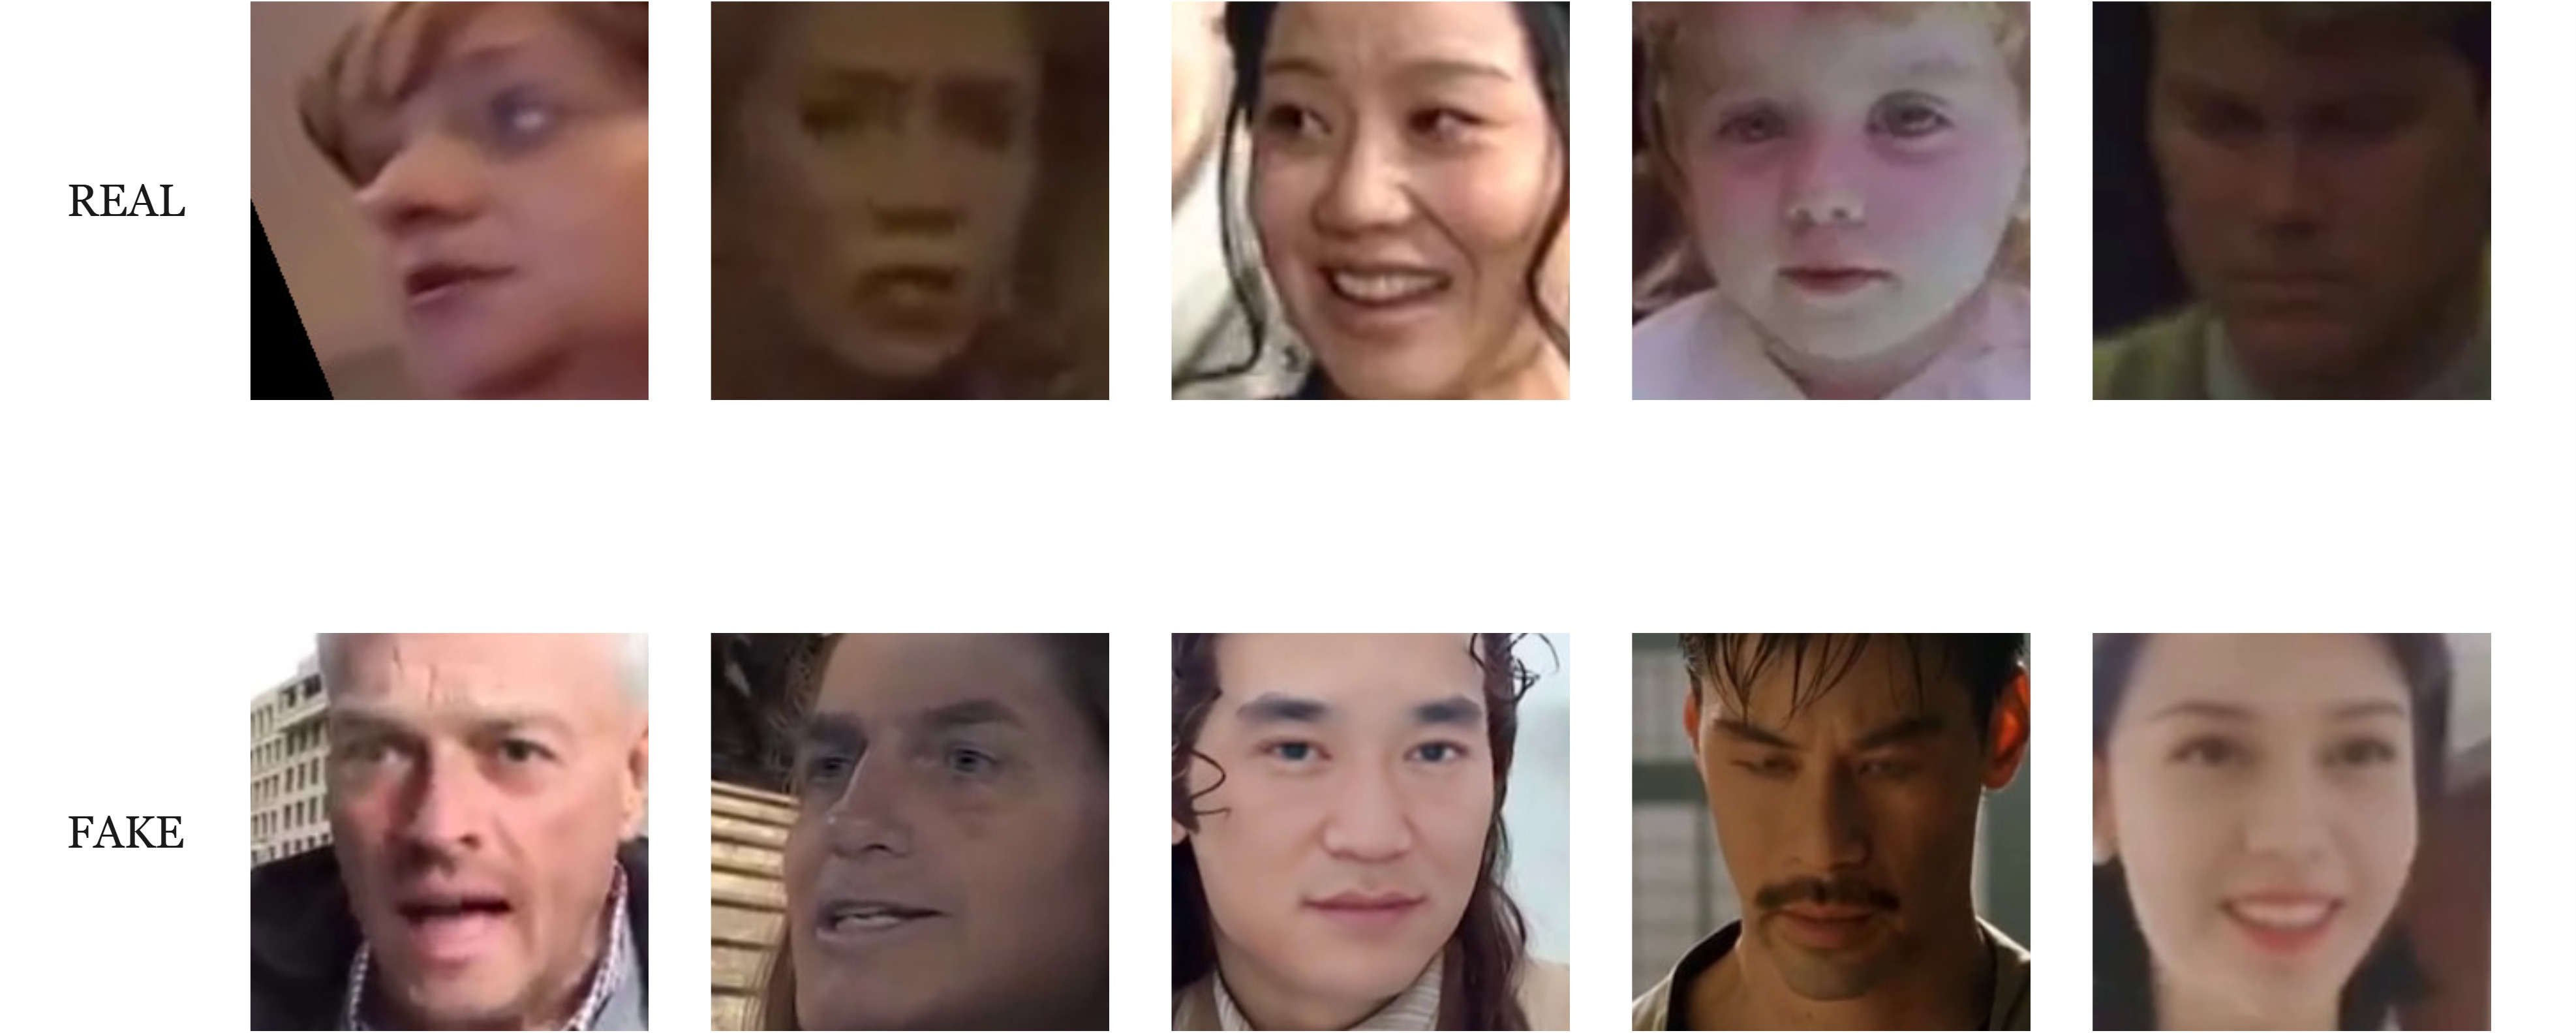
\includegraphics[width=0.7\textwidth]{figure/Sample WildDeepFake.jpg}
	\caption{Contoh Sampel Citra Wajah Kelas \textit{Real} dan \textit{Fake} pada Dataset \textit{WildDeepfake}}
	\label{fig:4.wilddeepfake-sample}
\end{figure}

\section{Hasil Pre-processing Data} \label{IV.Preprocessing}
Tahap pre-processing data dilakukan untuk menyiapkan dataset \textit{WildDeepfake} agar dapat digunakan sebagai masukan model. Pada tahap ini, data yang sebelumnya berbentuk sekuens wajah diproses menjadi klip dengan panjang seragam, kemudian dibagi ke dalam subset train, validasi, dan test.

\subsection{Hasil Pembentukan Klip 46 Frame} \label{IV.Klip46}
Pada tahap ini, setiap sekuens wajah pada dataset \textit{WildDeepfake} diproses menjadi klip turunan dengan panjang tetap 46 frame. Pembentukan klip dilakukan agar seluruh data memiliki panjang temporal yang seragam sebelum digunakan pada proses \textit{strided temporal sampling}. Dengan demikian, unit data yang digunakan pada tahap eksperimen bukan lagi sekuens wajah awal, melainkan klip wajah berdurasi tetap.

Potongan kode yang digunakan untuk membentuk klip 46 frame ditunjukkan pada Kode~\ref{code:4.1}.

\begin{lstlisting}[language=Python, caption={Pembentukan Klip 46 Frame}, label={code:4.1}]
CLIP_LEN = 46

def compute_centered_clip_ranges(num_frames: int, clip_len: int = 46):
	"""
	Menghasilkan rentang [start, end) untuk klip 46 frame.
	Strategi:
	- C = floor(N / L)
	- R = N - C * L
	- buang floor(R/2) frame di kiri
	- buang ceil(R/2) frame di kanan
	"""
	if num_frames < clip_len:
		return []

	num_clips = num_frames // clip_len
	used_frames = num_clips * clip_len
	remainder = num_frames - used_frames

	discard_left = remainder // 2
	start_idx = discard_left

	ranges = []
	for i in range(num_clips):
		s = start_idx + i * clip_len
		e = s + clip_len
		ranges.append((s, e))

	return ranges

def build_46f_clips_for_subset(
	extracted_subset_dir: Path,
	processed_subset_dir: Path,
	clip_len: int = 46
):
	reset_dir(processed_subset_dir)

	group_dirs = sorted(
		[p for p in extracted_subset_dir.iterdir() if p.is_dir()],
		key=lambda p: p.name
	)

	total_sequences = 0
	total_clips = 0
	skipped_sequences = 0

	for group_dir in group_dirs:
		group_id = group_dir.name
		out_group_dir = processed_subset_dir / group_id
		ensure_dir(out_group_dir)

		seq_dirs = sorted(
			[p for p in group_dir.iterdir() if p.is_dir()],
			key=lambda p: p.name
		)

		for seq_dir in seq_dirs:
			total_sequences += 1
			seq_id = seq_dir.name

			frame_files = list_image_files(seq_dir)
			n = len(frame_files)

			if n < clip_len:
				skipped_sequences += 1
				continue

			clip_ranges = compute_centered_clip_ranges(n, clip_len=clip_len)

			for clip_idx, (s, e) in enumerate(clip_ranges):
				clip_folder_name = f"{seq_id}_{clip_idx}"
				out_clip_dir = out_group_dir / clip_folder_name
				ensure_dir(out_clip_dir)

				selected_frames = frame_files[s:e]

				for frame_path in selected_frames:
					shutil.copy2(frame_path, out_clip_dir / frame_path.name)

				total_clips += 1

	return {
		"total_sequences": total_sequences,
		"total_clips": total_clips,
		"skipped_sequences": skipped_sequences,
	}
\end{lstlisting}

Kode~\ref{code:4.1} menunjukkan bahwa setiap sekuens terlebih dahulu dihitung jumlah klip penuhnya berdasarkan panjang klip 46 frame. Apabila terdapat sisa frame yang tidak membentuk satu klip penuh, sisa tersebut dibuang dari sisi kiri dan kanan secara seimbang. Setelah itu, setiap rentang frame disalin ke folder klip baru sehingga satu klip berisi tepat 46 frame.

Berdasarkan hasil pre-processing, diperoleh total 22.303 klip. Seluruh klip tersebut memiliki panjang 46 frame, sehingga tidak terdapat klip yang tidak valid. Distribusi kelas hasil pembentukan klip 46 frame ditunjukkan pada Tabel~\ref{table:4.klip46}.

\begin{table}[htbp]
	\centering
	\caption{Distribusi Kelas Hasil Pembentukan Klip 46 Frame}
	\label{table:4.klip46}
	\begin{tabular}{|c|l|r|}
		\hline
		\textbf{No} & \textbf{Kelas} & \textbf{Jumlah Data} \\
		\hline
		1 & \textit{Real} & 7.851 \\
		\hline
		2 & \textit{Fake} & 14.452 \\
		\hline
		\multicolumn{2}{|l|}{\textbf{Total}} & \textbf{22.303} \\
		\hline
	\end{tabular}
\end{table}

Berdasarkan Tabel~\ref{table:4.klip46}, jumlah klip kelas fake lebih banyak dibandingkan kelas real. Kelas fake terdiri atas 14.452 klip, sedangkan kelas real terdiri atas 7.851 klip. Hasil ini menunjukkan bahwa setelah sekuens wajah diproses menjadi klip turunan, distribusi data menjadi lebih didominasi oleh kelas fake.

\subsection{Hasil Pembagian Dataset} \label{IV.Split}
Dataset \textit{WildDeepfake} yang digunakan dalam penelitian ini sebelumnya telah memiliki pembagian awal berupa subset train dan test. Subset tersebut tersusun dalam empat direktori utama, yaitu \textit{real\_train}, \textit{fake\_train}, \textit{real\_test}, dan \textit{fake\_test}. Pada penelitian ini, subset \textit{real\_test} dan \textit{fake\_test} tetap digunakan sebagai data pengujian akhir. Sementara itu, data yang berasal dari subset \textit{real\_train} dan \textit{fake\_train} dibagi kembali menjadi data train dan data validasi.

Pembagian data validasi dilakukan dari subset train dengan rasio 80:20. Proses pembagian dilakukan pada level \textit{group\_id}, bukan pada level klip. Strategi ini digunakan agar klip turunan yang berasal dari sekuens atau sumber yang sama tidak terpisah ke subset yang berbeda. Dengan demikian, risiko kebocoran data antara data latih dan data validasi dapat dikurangi.

Potongan kode pembagian dataset ditunjukkan pada Kode~\ref{code:4.2}.

\begin{lstlisting}[language=Python, caption={Pembagian Dataset Train, Validasi, dan Test}, label={code:4.2}]
SEED = 42
VAL_RATIO = 0.20

# Data train resmi berasal dari subset real_train dan fake_train.
train_records = []
train_records += build_manifest_for_subset("real_train", subset_dirs["real_train"])
train_records += build_manifest_for_subset("fake_train", subset_dirs["fake_train"])

# Data test resmi berasal dari subset real_test dan fake_test.
test_records = []
test_records += build_manifest_for_subset("real_test", subset_dirs["real_test"])
test_records += build_manifest_for_subset("fake_test", subset_dirs["fake_test"])

train_df = pd.DataFrame(train_records)
test_df = pd.DataFrame(test_records)

# Split dilakukan pada level GROUP, bukan level klip,
# agar klip turunan seperti 101_0, 101_1, dan 101_2
# tidak terpisah ke subset yang berbeda.
group_df = (
	train_df[["group_id", "label", "label_name"]]
	.drop_duplicates()
	.reset_index(drop=True)
)

train_groups, val_groups = train_test_split(
	group_df,
	test_size=VAL_RATIO,
	random_state=SEED,
	shuffle=True,
	stratify=group_df["label"],
)

train_group_ids = set(train_groups["group_id"])
val_group_ids = set(val_groups["group_id"])

train_split_df = (
	train_df[train_df["group_id"].isin(train_group_ids)]
	.copy()
	.reset_index(drop=True)
)

val_split_df = (
	train_df[train_df["group_id"].isin(val_group_ids)]
	.copy()
	.reset_index(drop=True)
)

test_df = test_df.reset_index(drop=True)

# Validasi anti-leakage antara train dan validasi.
overlap_groups = set(train_split_df["group_id"]) & set(val_split_df["group_id"])

if overlap_groups:
	raise ValueError(
		f"Ditemukan kebocoran group antara train dan validasi: "
		f"{list(overlap_groups)[:5]}"
	)
\end{lstlisting}

Kode~\ref{code:4.2} menunjukkan bahwa data uji tidak dibagi ulang, melainkan tetap mengikuti subset test resmi dari dataset \textit{WildDeepfake}. Pembagian ulang hanya dilakukan pada subset train untuk membentuk data latih dan data validasi. Selain itu, penggunaan \textit{stratify=group\_df["label"]} bertujuan agar proporsi kelas \textit{real} dan \textit{fake} pada hasil pembagian tetap terjaga.

Hasil pembagian dataset berdasarkan subset dan kelas ditunjukkan pada Tabel~\ref{table:4.split}.

\begin{table}[htbp]
	\centering
	\caption{Hasil Pembagian Dataset Berdasarkan Kelas}
	\label{table:4.split}
	\begin{tabular}{|c|l|r|r|r|}
		\hline
		\textbf{No} & \textbf{Subset} & \textbf{Real} & \textbf{Fake} & \textbf{Total} \\
		\hline
		1 & Train & 5.376 & 10.124 & 15.500 \\
		\hline
		2 & Validasi & 1.382 & 2.189 & 3.571 \\
		\hline
		3 & Test & 1.093 & 2.139 & 3.232 \\
		\hline
		\multicolumn{2}{|l|}{\textbf{Total}} & \textbf{7.851} & \textbf{14.452} & \textbf{22.303} \\
		\hline
	\end{tabular}
\end{table}

Berdasarkan Tabel~\ref{table:4.split}, subset train memiliki jumlah data terbesar, yaitu 15.500 klip. Subset validasi terdiri atas 3.571 klip, sedangkan subset test terdiri atas 3.232 klip. Pada seluruh subset, jumlah klip kelas fake lebih banyak dibandingkan kelas real. Distribusi ini kemudian digunakan secara konsisten pada proses pelatihan, validasi, dan pengujian model.